\section{Method}
\label{sec:method}
We begin by introducing some notation and giving a brief overview of the multiple-instance tracking method introduced in \cite{lejeune18} that will serve as the base framework of this work. We then present our approach and highlight its integration in this framework.

\subsection{Base Framework}
The framework operates with a pre-segmentation of the image using standard superpixels~\cite{achanta2012} and assumes that each given 2D-point annotation indicates a location on the object of interest. By optiziming a max-flow graph (see Fig.~\ref{fig:ksp_network}), the entire sequence of images can be segmented from point-wise annotations. In \cite{lejeune18}, the annotations are used to model the likelihoods (costs) associated to the red, blue, and green edges of Fig.~\ref{fig:ksp_network}. In particular, two key models are to estimate these costs: (1) a transductive foreground model (blue arrows) and (2) a pairwise probability mode (red and green arrows). The full segmentation is then formulated as a Maximum a posteriori (MAP) problem, cast into a network flow problem, and solved using the edge-disjoint K-shortest paths algorithm \cite{berclaz11}; the latter being a multiple-instance tracking solver. We now detail both below (1) and (2):
\begin{figure}[t]
\centering
\includegraphics[width=1.\textwidth]{ksp_network}
\caption{Max-Flow graph (forward case). At each time frame $t$, a ``pseudo'' source node $\mathcal{E}_t$ is connected via an edge with flow $f_{t}^{\mathcal{E},n}$ (red) to tracklet $\mathcal{T}_t^n$. Each tracklet incurs a flow $f_t^n$ (blue) to visit superpixel $s_t^n$. Tracklets in frame $t$ are connected to tracklets in the next frame and allow for flows $f_{t}^{m,n}$ (green). The flow $f_{t}^{n,\mathcal{X}}$ can leave any tracklet in the network (orange).}
\label{fig:ksp_network}
\end{figure}

\textbf{Transductive Foreground Model: }
The transductive foreground model quantifies the cost associated with flow visiting a given superpixel, as depicted by the blue edges of Fig. \ref{fig:ksp_network}. Let the image sequence be denoted $\mathcal{I} = \{I_0,\ldots,I_T\}$ and let $\bm{g} = \{g_t\}_{t=0}^T$ with $g_t\in\mathbb{R}^2$ be a given 2D pixel location in $I_t$.
All images are assumed to be pre-segmented with $N$ superpixels $S_t=\{s^n_t\}_{n=0}^{N_t}$ using~\cite{achanta2012}.
In addition, each superpixel $s_t^n$ has appearance feature vector $z_t^n$ and $\bm{z}=\{z_t^n | t=0,\ldots,T,\quad n=0,\ldots,N_t\}$ is a set of all such feature vectors over all images.
Denoting the set $\mathcal{S}^p = \{s^n_t | g_t \in s^n_t, t=0,\ldots,T,n=0,\ldots N_t \}$ as all superpixels observed and the rest as $\mathcal{S}^u = \mathcal{S} \setminus \mathcal{S}^p$, as well as $\bm{Y} = \{Y_t^n|\forall(t,n)\}$ as the set of binary random variables such that $Y_t^n=1$ when superpixel $s_t^n$ belongs to the object, and $0$ otherwise. The objectness probability of all superpixels given all attended superpixels, denoted $\rho_{t}^n = P(Y_t^n = 1 | \bm{z}, \bm{g})$, is obtained by fitting a set of decision trees in a P-U learning scheme. This is achieved by averaging the votes of decisions trees.

\textbf{Pairwise Probability Model: }
Given two superpixels $s_t^i$ and $s_{t'}^j$, let $\alpha_{t,t'}^{i,j}$ define the probability that they are similar, whereby establishing a cost of either entering the network or transiting from one frame to the next (\ie depicted by the red and green edges of Fig.~\ref{fig:ksp_network}). In \cite{lejeune18}, $\alpha_{t,t'}^{i,j}$ are obtained via a supervised metric-learning where samples are split in a positive and negative set by thresholding on $\bm{\rho} = \{ \rho_t^n | \forall(t,n)\}$
 and then using Fisher Discriminant Analysis \cite{welling05} to maximize inter-class variance and minimize intra-class variance.

\subsection{A Deep Embedded Clustering Approach}
\label{sec:dec}
While the above methods were shown to be effective, they suffer from the fact (1) that the feature encoding component is decoupled from the similarity metric optimization component and (2) the superpixel similarity measure $\alpha_{t,t'}^{m,n}$ is taken as a simple Gaussian distance in the feature space, which ignores the potential presence of sub-populations (clusters). In the following, we describe our contribution which focuses on modeling of the likelihoods (costs) associated to the red, blue, and green edges of Fig.~\ref{fig:ksp_network}.

Our approach to model these costs is inspired by the Deep Embedded Clustering (DEC)~\cite{xie15} that optimizes for the similarity metric and the feature encoding jointly, and which allows us to leverage a sequence-specific distance between clusters. We now describe in detail our approach which is illustrated in Fig.~\ref{fig:network} and consists of two components: (1) an initial feature learning model that learns a representation and (2) a self-supervised clustering method which allows efficient similarity estimation between image regions. In our approach, both are learned end-to-end.
\begin{figure}[b!]
\centering
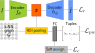
\includegraphics[width=0.79\textwidth]{network2.png}
\caption{The top row is a convolutional neural network configured for autoencoding. Features are pooled on regions of interest (Superpixels) and projected to a low dimensional space via a fully connected layer (FC). The soft assignments $q$ are then optimized to their hardened target assignments $p$.}
\label{fig:network}
\end{figure}

\subsubsection{Feature encoding: }{
  Using a traditional encoder-decoder approach for image reconstruction, our network computes a latent space representation at each pixel.
  Given that our graph operates on a superpixel representation, we use average-pooling on the feature map on all pixels belonging to a superpixel (ROI pooling) and then use a low-dimensional projection, via a fully connected layer, to have a compact representation $z_i$.
}

\subsubsection{Self-supervised clustering: }{ 
We hypothesize that our objects of interest are aggregations of superpixels that potentially span several frames. We assume that a single annotation point is given per frame and wish to train a model that will give a measure of similarity of the given sample with its neighbors. Ideally, we wish to assign  $v_i$ to clusters such that each cluster has low intra-variance. 

Let $\bm{\mu}=\{\mu_j \in V\}_{j=1}^k$ be a set of $k$ centroids lying in the feature space $V$.
Letting $v_i$ the dimensionally reduced feature vector that corresponds to $z_i$, a similarity to centroid $\mu_j$ computed by the student's t-distribution,
\begin{equation}
q_{ij} = \frac{(1 + ||v_i - \mu_j ||^2)^{-1}}{\sum_{j'}(||v_i - \mu_{j'} ||^{2})^{-1}}.
\label{eq:soft_assign}
\end{equation}
}
\noindent
Note that Eq.~\eqref{eq:soft_assign} is a soft version of a typical K-means cluster assignment (\ie $q_{ij}$ are not binary as in K-means). From Eq.~\eqref{eq:soft_assign}, we can derive a target distribution that aims at hardening this t-distribution,
\begin{equation}
p_{ij} = \frac{q_{ij}^2 / f_j}{\sum_{j'}q_{ij'}^2/f_{j'}}
\label{eq:tgt_assign}
\end{equation}
\noindent
where $f_{j}=\sum_i{q_{ij}}$.
Hence, the distribution $p_{i}$ is a more strongly peaked distribution to that of $q_{i}$ and our objective is to learn the centroids $\mu_j$ such that $p_{i}$  and $q_{i}$ are similar to each other, while simultaneously changing $V$ to achieve this.
We detail how to optimize this next.

\subsubsection{Optimization: }{ 
To learn $v_i$ and $\bm{\mu}$, we first use a pre-training phase to optimize a reconstruction loss between the input images $I$ and the reconstructions $\hat{I}$ using a standard encoder-decoder architecture:
\begin{equation}
\mathcal{L}_r = \frac{1}{|I|}\sum_{k,l} ||I(k,l) - \hat{I}(k,l)||^2.
\label{eq:loss_recons}
\end{equation}
\noindent
In a second stage, we use a clustering purity loss that will harden our clusters towards their targets using the Kullback-Leibler divergence:
\begin{equation}
\mathcal{L}_c = D_{KL}(P||Q),
\label{eq:loss_sim}
\end{equation}
\noindent
where $Q$ is a batch of soft-assignments $q_{ij}$ and $P$ the corresponding targets $p_{ij}$.
The complete loss function then optimizes for both cluster purities and the reconstruction loss so as to restrict the distortion of the feature space:
\begin{equation}
\mathcal{L} = \mathcal{L}_c + \gamma \mathcal{L}_r.
\label{eq:loss}
\end{equation}

\subsubsection{Implementation and training: }{ 
  The autoencoder used is a Deeplabv3+ architecture~\cite{chen17} with Dilated Residual Network (DRN) as backbone~\cite{yu17}. 
In contrast with the original architecture, we remove the skip connection that includes the low-level features of the encoder at the input of the decoder. The Deeplabv3 architecture combines the latter output to a dilated spatial pyramid pooling module to extract feature maps in parallel at different spatial scales. By concatenating these, we obtain a feature map that better captures multi-scale context. We use the method described~\cite{schuurmans18} for the ROI pooling module.
  
The autoencoder is pre-trained with data augmentation for $100$ epochs and a learning rate of $10^{-1}$.
In its original formulation, DEC is inherently unstable as all target distributions $\bm{q}$ are modified at each gradient descent iteration \cite{guo17}.
We therefore implement a buffer that stores the targets of all samples before training.
The targets are then updated for all samples every $T=10$ epochs.
Before the clustering phase, we compute the soft-assignment module with $K=15$ centroids using the K-means algorithm.
Likewise, the dimensionality reduction layer is initialized in a similar fashion as~\cite{lejeune18} to $15$ dimensions.
The encoder, decoder, centroids, and fully connected layer are optimized for $200$ epochs with a learning rate $10^{-3}$ and $\gamma=0.1$.
All sequences are pre-segmented into $\sim 1200$ superpixels per-frame.
}

\subsubsection{Clustering-based pairwise probability model: }{ 
Once trained, we use the optimized centroids $\bm{\mu}$ as follows. We assign each sample $v_i$ to a cluster $c_i=\arg \max_{j}q_{ij}$.
We then fit a Gaussian mixture model on all samples by taking as initial means $\bm{\mu}$, component weights $\bm{\pi}=\{\pi_j|\pi_j=|c_j|/N\}$, and covariance matrices $\Sigma_j=cov[\bm{v_j},\bm{v_j}]$. By letting $p(v_i) = \left[ \cdots \pi_j \mathcal{N}(v_i|\mu_j,\Sigma_j)\cdots \right]$ be the posterior probabilities of sample $v_i$, we can then compute the pairwise similarity of $v_i$ and $v_{i'}$ as the Bhattacharya coefficient of $p(v_i)$ and $p(v_{i'})$,
\begin{equation}
BC_{ii'} = \sum_{k=1}^K{\sqrt{p(v_i)_k p(v_{i'})_k}}.
\label{eq:bc}
\end{equation}
}
\noindent
Eq.~\eqref{eq:bc} thus provides the costs associated to the green and red edges in Fig.~\ref{fig:ksp_network}.
%%% Local Variables:
%%% mode: latex
%%% TeX-master: "00_main"
%%% End:
